%% heading for this chapter
This chapter outlines and highlights useful background that will be explored in further detail in upcoming chapters as well as provides an outline for the thesis.

We begin with an overview of the standard model, and how both its success and short comings drive larger and more expensive detectors.
These detectors must reach for ever newer limits, in both precision and scale, due to the robust nature of the Standard Model.
To elucidate the issues at the forefront of the Standard Model we provide a brief history, with an emphasis on the detectors and experiments which helped lead to its current status.
Next, we become more specific and discuss DUNE which is a example of a new, large, and expensive detector which aims to push beyond the Standard Model.
Finally, we finish this section on a discussion on the developments of new tracking detectors and highlight their relevance to the work presented here.

%% Where we are
\section{The State of Things: The Standard Model}
~\label{sec:intro_now}

What is the universe made of?
What are the fundamental building blocks of matter?
Since time immemorial thinkers have questioned the nature of the universe and wondered what the basic building blocks of nature are.
The answer to these fundamental questions is the motivation for particle physics.

%% what is the SM: Summarize what it does well and what it doesn't do well
In the history of science, it is easy to argue that the most successful of all models is the Standard Model of Physics.
The Standard Model (SM)~\citep{GLASHOW1961579, salam1964electromagnetic, weinberg1967model} was originally developed in the mid to late 1970's and is the model responsible for unifying the weak, strong, and electromagnetic forces together.
It was gradually developed in the 1970's as a result of the boom in particle detectors in the mid and late 1960's.
It has made remarkable predictions about the existence of elusive neutrinos, quarks and vector bosons before their discovery, and more.

The comprehensive and extensive list of known particles as well as various cross-sections, lifetimes, and other known information can be found from the bi-annually published Particle Data Group (PDG)~\citep{Workman:2022ynf}.
The SM has been experimentally tested to limits unlike any other theory.

In this section we briefly describe the SM and highlight some (certainly not all) key aspects of its formulation as understood today.
The SM has stood the test of time, despite many known failures and holes in its predictions.
Therefore, we hope to elaborate a bit on its status involving predictions and unknwon parameters to help the reader better appreciate the significance of looking for physics beyond the SM.

\subsection{The Basics of the Standard Model}

The SM itself dictates what the fundamental constituents of matter and energy are.
Like any theory in science, its purpose is to explain observed phenomena.
In this case, the observed phenomena are not simply the origin of all observable particles and their masses, but also a description of all observable interactions.

The interactions described by the SM involve the fundamental particle interactions via three of the four known fundamental forces observed in nature: the electromagnetic, weak, and strong forces.
The missing fourth force is one of the major shortcomings of the SM: its inability to incorporate a quantum description of gravity.
The discussion of the renormalization of quantum gravity is beyond the scope of the work presented here, so we will only mention that it needs to be achieved.

All currently known fundamental particles are represented in Fig.~\ref{fig:cern_sm}.
These particles represent the today's best knowledge of the building blocks of all observed matter in the universe.

\begin{figure}[]
\centering
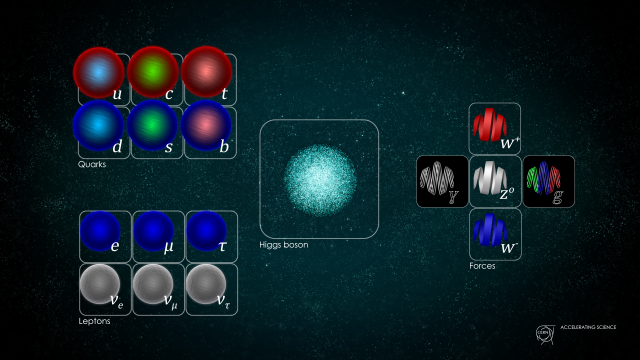
\includegraphics[width=\textwidth]{images/STDM_higgs_and_field_D.png}
\caption{Image of Fundamental Particles in the Standard Model, taken from CERN website~\citep{dominguez_2015}.
  All known matter and particle interactions involves combinations of the particles shown here.}
\end{figure}
~\label{fig:cern_sm}

\subsubsection{The Quarks}

The quarks represent particles in the top left of Figure~\ref{fig:cern_sm}.

Quarks are the fundamental particles which constitute the ``normal'' heavy particles, such as protons and neutrons.
The quarks also have unique anti-particle partners, which brings the total number of quarks up to 12.
Like all antiparticles, the anti-quark partners have the same mass as the normal partners, with all the quantum numbers reversed.

A unique feature of quarks compared to leptons is that no ``free'' quark has ever been observed.
This means that all current direct observations of quarks are in bound states.
Most commonly, the quarks combine in pairs or triplets to form mesons and baryons, respectively.
Even more complicated assemblies can be made of additional quarks, such as tetra and penta quarks, as long as all the quantum numbers are unique for each quark.

The mesons contain a quark and an anti-quark, whereas the baryons a contain three quarks.
Collectively, all particles constituted by any combination of quarks are known as hadrons.
In 1961 Murray Gell-Mann proposed his ``eight-fold way''~\citep{eightfold_way_osti_4008239} which provided a method of grouping the hadrons.

Since quarks are not freely observable a common place to infer their existence (and to create heavier hadrons) are in particle accelerators.
The most well known particle accelerator is the Large Hadron Collider (LHC) in Geneva.
These Particle accelerators generate extremely high energy ($\approx \mathcal{O}(10 TeV)$) protons which when collided can generate new composite hadrons of any mass so that the total energy is conserved.

Since quarks, due to their color, readily combine to create more easily observed composit particles.
The Quark model was then propossed by Gell-Mann in 1964~\citep{quark_model_GELLMANN1964214}.
This model is a group theory concept (known as SU(3) symmetry) and is the means for which the fundamental particles (quarks) combine into the composite particles (hadrons) which are more readily and easily measured today.
Eventually experiments conducted at the Stanford Linear Accelerator (SLAC) between 1967-1973 verified the existence of these quarks and Gell-Mann won the Nobel Prize in 1969.

The rescue of the quark model came with the measurement of~\citep{Jpsi_PhysRevLett.33.1404}.
The $J/psi$ particle indicated the existence of a fourth since then unmeasured quark, which we now know as the charm ($c$).

\begin{table}
\begin{center}
\begin{tabular}{||c c c c c||}
 \hline
 Quark & Charge & Mass (MeV) & Year Discovered & Ref.\\ [0.5ex]
 \hline\hline
 up & $\frac{2}{3}$ & 2.16 & 1968 & SLAC~\citep{1969PhRvL..23..930B, 1969PhRvL..23..935B} \\
 \hline
 down & $\frac{-1}{3}$ & 4.67 & 1968 & SLAC~\citep{1969PhRvL..23..930B, 1969PhRvL..23..935B} \\
 \hline
 strange & $\frac{-1}{3}$ & 93.4 & 1968 & SLAC~\citep{1969PhRvL..23..930B, 1969PhRvL..23..935B} \\
 \hline
 charm & $\frac{2}{3}$ & 1270 & 1974 & SLAC~\citep{Jpsi_PhysRevLett.33.1404} \\
 \hline
 bottom & $\frac{-1}{3}$ & 4180 & 1977 & Fermilab~\citep{bottom_PhysRevLett.39.252}\\
 \hline
 top & $\frac{2}{3}$ & 173000 & 1995 & Fermilab~\citep{topquark_Abachi_1995} \\
 \hline
\end{tabular}
\caption{Description of the discovery of quarks.
  Notice that as the mass increases for a particular quark the year of discovery also increases.
  This is a property of how we create and observe the quarks in our accelerators, and also the reason why physicists continue to want to build bigger ones.
  Interesting physics happens at higher and higher energies, which require larger and more expensive detectors to probe these energy scales.
  Note that the lighter quark masses are not well understood for other experimental reasons, and the presented data are rounded to three significant figures based on~\citep{Workman:2022ynf}.}
\end{center}
\end{table}
~\label{table:quark}

%% TODO
\subsubsection{The Leptons}

The leptons represent particles in the bottom left of Figure~\ref{fig:cern_sm}.

The first lepton discovered, and the most commonly recognized, is the electron which was discovered by J. J. Thomson.
Just like the quarks, the leptons come in three families (electron, $\mu$, $\tau$).
Also like the quarks, the leptons have charge, mass, and flavour which means they can decay.

Unlike the quarks the leptonic particles do not have a color quantum number and therefore do not combine together to create composite particles.
Additionally, free leptons are observed, e.g. the electron.

The most difficult to measure fundamental particles of within the SM are the neutrinos.
This is because these leptons carry no net charge.
However, since they carry flavour and can decay (or be absorbed) and they also carry their respective lepton number, the neutrinos in the family can be identified by measuring their partner.

For example, a common process to observe an anti-electron neutrino ($\hat{\nu_{e}}$) is through inverse beta-decay (IBD) following the reaction:
\begin{equation}
\hat{\nu_{e}} + p \rightarrow e^{+} + n
\end{equation}

This IBD reaction is a common measurement tool for identifying neutrinos because of the distinguisable detection signature of the produced particles.
The position ($e^{+}$) annailates quickly ($\approx \mathcal{O}(ns)$) and will produce back-to-back 511 $keV$ photons.
The produced neutron, on the other hand, wobbles around much longer ($\mathcal{O}(us)$) before being captured, which produces scintillation light of energy proportional to the neutrons energy when captured.

The muon ($\mu$) was discovered by Anderson and Neddermeyer in 1936 by observing cosmic ray showers~\citep{muon_discovery_PhysRev.51.884}.

The tau ($\tau$) was discovered by SLAC in 1975~\citep{tau_discovery_PhysRevLett.35.1489}.

The first measurements of the neutrinos in each family were much harder than their charged partners.
The electron neutrino ($\nu_{e}$) and the muon neutrino ($\nu_{\mu}$) are observed in decay interactions.

The tau neutrino ($\nu_{\tau}$) was exceptionally difficult to measure.
Like the previous neutrino partners, the $\nu_{\tau}$ is discovered by looking for the creation of its partner ($\tau$) during a CC interaction.
As a comparison the $\tau$ has a lifetime of only $10^{-13}$ s whereas the muon life time $T_{\mu}\approx \mathcal{O}(1 \mu s)$ or seven orders of magnitude shorter!

The first successful experiment came in 2000~\citep{tau_neutrino_discovery_KODAMA2001218}.
DONUT utilized a much more complicated emulsion detector to collect tracks from a 800 GeV proton beam offline.
The exxperiment collected a total of 203 neutrino interactions, of which it found evidence for a total of only four interactions.

\begin{table}
\begin{center}
\begin{tabular}{||c c c c c||}
 \hline
 Lepton & Charge & $N_{e}$ & $N_{\mu}$ & $N_{\tau}$ \\ [0.5ex]
 \hline\hline
 $e^{-}$ & 1 & 1 & 0 & 0 \\
 \hline
 $\nu_{e}$ & 0 & 1 & 0 & 0 \\
 \hline
 $\mu$ & 1 & 0 & 1 & 0 \\
 \hline
 $\nu_{\mu}$ & 0 & 0 & 1 & 0 \\
 \hline
 $\tau$ & 1 & 0 & 0 & 1 \\
 \hline
 $\nu_{\tau}$ & 0 & 0 & 0 & 1 \\
 \hline
\end{tabular}
\caption{Description of the quantum numbers of the fundamental lepton families.
  There are three unique families within the leptons: electron, muon, and tau.
  The charge carrier as well as the neutrino each carry a value of one for this number.
  Their anti-particle counterparts carry -1 of this number.}
\end{center}
\end{table}
~\label{table:lepton_qn}

\subsubsection{The Forces - Vector Bosons}

All forces within the standard model (electromagnetism, weak, and strong) are governed via a ``carrier'' particle.
These carrier particles are represented on the center-right of~\ref{fig:cern_sm}.

The electromagnetic force is governed by particle exchanges of a photon.
Other than perhaps gravity, which isn't explained by the SM, this is the most well known and described force.
All particles which carry charge  interact via this force.
Therefore the neutrinos are the only particles within the quarks and leptons which do not interact at all with the electromagnetic force (this is why detecting them is so hard).
The full theoretical description of this force is governed by Quantum-Electrodynamics (QED).

The weak-nuclear force is governed by particles exchanges of one of the three particles in the center: $W^{\pm}$ and $Z$.
This force involves a change in flavor of a particle, and involves both quarks and leptons.
It is also responsible for all decay processes.
The theoretical description of these mechanics are called Quantum-Flavourdynamics (QFD).

The strong-nuclear force is governed by the exchange of the gluon ($g$).
This force is responsible for color changes of matter and describes why nuclei are held together.
Since this force only involves exchanges of a gluon, the leptons are therefore unaffected since these particles carry no color quantum number.
The full theoretical description for the strong-nuclear force is Quantum-Chromodynamics (QCD).

The gluon was discovered in at the TASSO experiment 1979~\citep{tasso_1978_BRANDELIK1979243, PETRA_PhysRevLett.43.830}.

Measurements of the intermediate bosons were much harder.
The $W^{\pm}$ boson were measured in 1983~\citep{wboson_measure_ARNISON1983103}.
Followed by the Z boson which was measured shortly afterwards in the same experiment~\citep{zboson_measure_1983398}.

\begin{table}
\begin{center}
\begin{tabular}{||c c c c c||}
 \hline
 Force & Scale & Theory & Carrier & Ref. \\ [0.5ex]
 \hline\hline
 Strong & 10 & Chromodynamics & gluon & TASSO~\citep{tasso_1978_BRANDELIK1979243} \\
 \hline
 Electromagnetic & $10^{-2} $ & Electrodynamics & photon & Planck? \\
 \hline
 Weak & $10^{-13}$ & Flavourdynamics & $W^{\pm}$,Z & CERN~\citep{wboson_measure_ARNISON1983103},\citep{zboson_measure_1983398}\\
 \hline
 Gravity & $10^{-42}$ & General Relativity & graviton  & ?? \\
 \hline
 \hline
\end{tabular}
\caption{Relative strength chart of the four fundamental fources of nature. Although gravity is not included within the SM it is included, as well as its theoretical force carrier the graviton.}
\end{center}
\end{table}
~\label{table:forces}

\subsubsection{The Higgs - Scalar Boson}

The last particle to be discovered in the SM was the Higgs particle.
The Higgs particle was originally predicted in 1964 by Peter Higgs~\citep{HIGGS1964132}.
This particle is important to describe how mass is given the the elementary particles described by the SM.
Finally, in 2012 the Large Hadron Collider (LHC) was able to infer the massive Higgs particle~\citep{higgs_discovery_20121}.

%% elaborate more here on the standard model, what is it really?
\section{The Problem: Moving Beyond the Standard Model}

Despite its (SM) numerous achievements in predictive power and experimental verification we know today that it has crucial shortcomings.
The Standard Model (SM)~\citep{GLASHOW1961579, salam1964electromagnetic, weinberg1967model} has no ability to account for Dark Matter or Dark Energy in the universe, nor the distribution (or the hierarchy) of neutrino masses, nor is it able to relate how gravity interacts with the other fundamental forces of nature (Unification).
It also doesn't account for some 'basic' properties it has, such as: why are there only three generations of leptonic particles (electron, muon, and tau)?
These short-comings offer hints for where to search for physics.
Physicists have known about these short comings from the conception of the Standard Model and have (to no avail) sought out what's next.

With a plethora of hints to search for New Physics (NP), it can be useful to organize the efforts of search.
In 2008 the Particle Physics Project Prioritization Panel (P5) did just this and labeled the three frontiers of physics: the cosmological, energy, and intensity frontiers.
Each of these frontiers offer different kinds of challenges and serve as guides to look for physics beyond the SM.

\begin{figure}[]
\centering
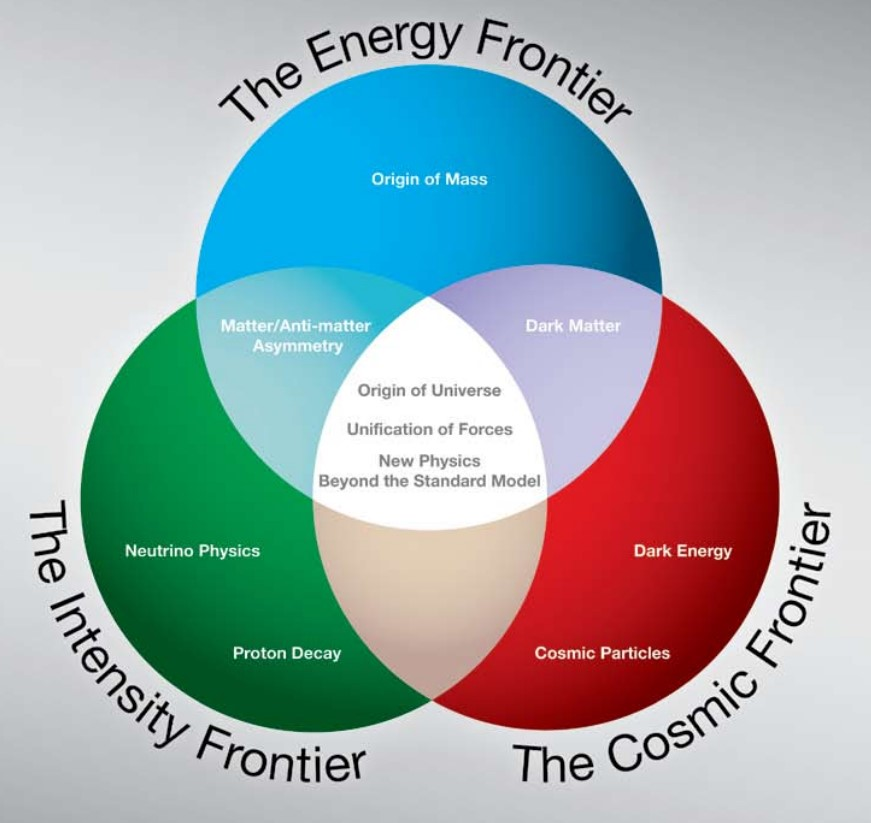
\includegraphics[width=0.5\textwidth]{images/frontiers_physics.jpg}
\caption{Image based on the 2008 P5 report~\citep{intensityfrontier2012_Hewett}. The white text labeled within each frontier describes the search for some physics beyond the SM within that frontier.}
\end{figure}

%% energy frontier problems
\subsubsection{Searches at High Energy}
The energy frontier is concerned with the origin of mass.
The Large-Hadron Collider (LHC)~\citep{higgs_discovery_20121} experiment is the archetypal experiment aimed at solving problems within this frontier.
The LHC itself consists of other large-scale tracking and calioremtry experiments such as ATLAS~\citep{ATLAS:1999vwa} and CMS~\citep{CMS:2006myw}.

Large particle accelerators are used to generator source particles of ever increasing energy.
Due to the conservation of mass, the higher the energy of the particle accelerated the higher the mass (energy) of the particles created after certain collisions can be.

There also exist lepton collidors~\citep{belle2_tdr_arxiv} which offer unique areas of search along this frontier too.
More detailed descriptions of such collider experiments are beyond the scope of the work presented here, and further reading may be pursued from the extremely detailed technical design reports cited here of Belle-II and the ATLAS experiments.

%%
\subsubsection{Other Searches}
The cosmological frontier aims to search for NP on extremely large time and distance scales by relying on observational techniques.
Cosmological measurements have shown the that majority of the universe's matter is not visible to light, and so we call it dark matter.
Additionally, the universe is expanding at an accelerated rate, which we can tell from the blueshift of distance galaxies.
Likewise, cosmologists have also discovered that the universe is expanding due to some invisible energy in the universe, and so we call it dark energy.

The search for these dark causes of the universe lie within the realm of the cosmological frontier.

Dark energy currently resides as the explanation for the observed accelerated expansion of the universe.
Dark matter is commonly used to explain the deviation of the rotational frequency of galaxy clusters.

The third (and final) frontier we'll discuss is the Intensity frontier.
The Intensity Frontier of Physics (\citep{intensityfrontier2012_Hewett}) is one which today requires very large and very precise measurements to gain the statistics to declare an observation.
In order to address the issues posed within this frontier the large scale detectors hunting for New Physics (NP) have continued to grow in size, energy sensitivity, and importantly cost: \citep{Juno:2022103927}.

As compared to the energy frontier which normally relies on creating new particles from accelerators the Intensity Frontier often searches for rare events, like a proton decay.

Neutrino searches also lie within this frontier.
Neutrinos are notoriously difficult to detect and measure since they can only be probed via the weak-nuclear force, and even then only indirectly since they carry no charge themselves.

%%
\subsection{How did we got here?}

Many times since the early 20th century it was thought that the goal of physics was accomplished.
However, during each of these moments of false triumph some new detector was built to take a new measurement; thus, the door to new understanding of nature is never closed.
This section provides a brief and (necessarily) incomplete history of significant measurements and detector developments relevant to particle physics in the creation of the SM.
In order to clear an obstacle, it is often helpful to remember the previous ones.


\subsection{A Century of New Physics}

At the turn of the 20th century particle physics was in its infancy.
In 1900 Max Planck first introduces the concept of energy quanta for the first time concerning photons to eliminate the infamous ultra-violet catastrophe problem introduced by statistical mechanics.
JJ Thomson used a single cathode-ray tube to discover the electron and the nucleus, and won for himself the Nobel Pize in 1906.
Milikan's famous oil-drop experiment won him the Nobel Prize in 1923.

However, as each of these new discoveries solved problems only more questions were produced.
Once the nucleus was discovered to contain only protons and neutrons, the natural question arose: what holds all of the positive charge together in the center.
Thus, physicists cleverly named the new force which was stronger than the electromagnetic force: the Strong Force.

The bubble chamber was then invented in 1952 by Donald Glaser~\citep{bubbleChamber_PhysRev.87.665}.
These detectors proved significant in the discover of the W and Z bosons and ultimately allowed the unification of the electromagnetic and weak forces to form the electroweak theory.

Next the spark chamber eventually lead to the gradual development of the wire-spark chamber.
In 1968 Georges Charpak developed the Multi-Wire Proportional Chamber (MWPC) for which he (much later) won the Nobel Prize in 1992.
From this key insight a new detector concept was made possible.

\subsection{Finding Neutrinos}
~\label{sec:neutrinos}

Hints at the existence of neutrinos began early last century.
More than 100 years ago Chadwick was able to show that the energy spectrum from a decaying electron was continuous~\citep{Chadwick:1914zz}.
This unknown cause of the spectrum even lead some physicists to belief that perhaps the conservation of energy was violated.
Wolfgang Pauli instead predicted a particle which he originally called the neutron to also be a decay product, but not easily observable.
This third particle in the decay would explain the energy spectrum of the electron.
Quickly however the particle name neutron was taken by a different neutral particle in 1932~\citep{Chadwick1932PossibleEO}
The discovery of the neutron and the continuous spectrum of beta decay forced Pauli to come up with a new theory attempting to describe beta decay~\citep{pauli_1934}.

Originally physicists held little hope that such an elusive particle would ever be detected.
However, the motivation to save this conservation law lead Wolfgang Pauli to the first prediction (1930) of the neutrino; the reason that the energy was a spectrum from the electron was that some of the energy was ``taken up'' by the neutrino.
Finally, some 26 years later in 1956 was the first observation of the electron neutrino~\citep{first_neutrino_measurement}.

The discovery of the electron neutrino $v_{e}$ was the first of the three families to be discovered.
A few years later the first reactor neutrino ($\nu_{\mu}$) was observed at Brookhaven National Laboratory (BNL)~\citep{PhysRevLett.9.36}.

The first measurement of the $\tau$ neutrino ($\nu_{\tau}$) happened much later in 2001~\citep{tau_neutrino_discovery_KODAMA2001218}.
this detector used nuclear emulsions.

Daya Bay~\citep{daya_bay_2012_neutrino_PhysRevLett.108.171803} has also established measurements of electron anti-neutrino ($\bar{\nu_{e}}$) disappearance.

% Super-K / SNO / KamLand / NOvA / daya bay / RENO / double chooz / t2k / minos
After this first discovery is when the the answers, followed by more questions, came.
Since then, many large-scale experiments have been dedicated to measuring the three generations of neutrinos.
~\citep{SNO_2002_neutrino_PhysRevLett.89.011301,
neutrino_measurement_NOvA_2019_prl,
t2k_2011_neutrino_PhysRevLett.107.041801,
reno_2012_neutrino_PhysRevLett.108.191802,
FUKUDA2002_solar_neutrino_oscillation,
kamland_2003_neutrino_PhysRevLett.90.021802,
daya_bay_2012_neutrino_PhysRevLett.108.171803,
doubleChooz_2012_neutrino_PhysRevLett.108.131801}

All reliable information we have about neutrinos come from these large scale detectors.

Originally the mass of the neutrino predicted by the SM was massless.
That was until the Solar-neutrino anomaly measured significantly less neutrinos than predicted~\citep{solar_neutrino_problem_PhysRevLett.20.1205}.
The solution for this was oscillation.

\section{Modern Tracking Detectors}

It is could said that any definition defining a ``new'' age of a types of detectors is subjective.
Nevertheless, we proceed to define that modern particle detectors were the age that began to use modern electronics, or electronics after the development of the metal–oxide–semiconductor field-effect transistor (MOS-FET).
If there was any invention which was able to drive the development of computers and  measuring electronics, it was the transistor.
Therefore, the beginning of the modern particle detection age began with the transistor, and it saw to the end of the spark chamber and bubble chamber detectors.

\subsection{Multi-Wire Proportional Chamber}

The middle of the 20th century saw a dramatic increase in the ability and reduction of the cost of electronics.
These (then) new electronics allowed for fast digitizing measurements of voltage or current.
Thus, new propotional counter detectors were capable of using computers to do the measuring or counting of the events within the detector.
The rate at particles could then be detected increased by orders of magnitude.

Using the fast digitizers and closely spaced wires Georges Charpak (1924-2010) created the firstWire MWPC in 1968~\citep{Charpak:1968kd}.
This new detector was one which paved the way for modern detector development, for which Charpak won the 1992 Nobel Prize.


\subsection{Time Projection Chambers}

Time Projection Chambers (TPC)~\citep{lartpc:nygren} have been shown to be extremely useful in high energy physics experiments due, in part, to their high resolution in both timing and spatial dimensions.
This detector was originally used in the Position-Electron Project PEP-4 experiment which measured electron-positron collisions from the 29 GeV electron beam produced at the Stanford Linear Accelerator (SLAC).
The first TPC design used high pressure gas and was able to measure 1000s of particle tracks per second (compared to 1-10) and provide full 3-D event reconstruction.

It did not take long for other experimentalists to generalize this concept to different elements or even to liquid.


\subsection{Noble Gases and Time Projection Chambers}

The technology of TPCs has greatly matured since their original inception.
in many kinds of detectors across HEP. TPCs can also incorporate two phases of a substance (liquid and gas), called Dual Phase (DP) TPCs.

the Xenon-1T is a dark matter experiment which is a dual-phase TPC \citep{Aprile_2017_xenon1T}.

\begin{figure}[]
\centering
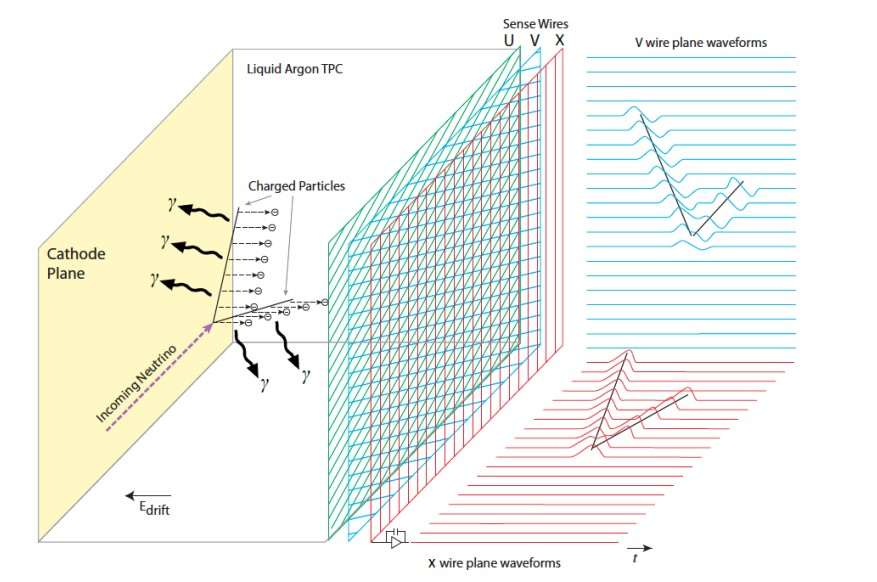
\includegraphics[width=\textwidth]{images/dune_tdrv12020_lartpc-sp.jpg}
\caption{Image of a Time Projection Chamber (TPC).
Charge is accumlated within the volume as ions are removed from the fidicial volume from another charged ion as it passes through the material.
An uniform electric field drifts the free now electrons towards the anode plane.
The collection and readout of charge on this anode plane is what is recorded within the detector.
Image is taken from~\citep{DUNE_TDR_V1_Abi_2020}.}
\end{figure}~\label{fig:dune_apa}

The LUX experiment is a single phase TPC also hunting for dark matter.

A specific kind of TCP is a Liquid Argon Time Projection Chamber (LArTPC)~\citep{rubbia1977liquid}.

%% include relevant LArTPCs here
Recent work on LArTPCs (\citep{ArgoNeuT_PhysRevD.99.012002, MicroBooNE_Acciarri_2017, LArIAT_Acciarri_2020}.)

Energy resolution of the LArTPCs within DUNE are still unknown to within a factor of 4 \citep{lartpc_energy_resolution:PhysRevD.99.036009}.

%% LAr table
\begin{table}
  \begin{center}
    \begin{tabular}{||c c c c||}
 \hline
      Property & Symbol & Value & Unit \\
 \hline\hline
      Density & $\rho$ &  1.3973 & $g cm^{-3}$ \\
      Fano Factor & F & 0.107 & - \\
      Dielectric Constant & $\epsilon$ & 1.505 & - \\
      electron drift velocity & $v_{e}$ & 0.1601 & $\unit{cm/\mu s}$ \\
      Ionization Energy of single $e^{-}$ & $W_{i}$ & 23.6 & eV/$e^{-}$ \\
      Ionization Energy of single $e^{-}$ from photon & $W_{scint}$ & 19.5 & eV/$\gamma$ \\
      Minimum Specific energy loss & $(dE/dX)_{MIP}$ & 2.12 & MeV/cm \\
      Hadronic Interaction Length & $\lambda_{int}$ &85.7 & cm \\
      Scintillation Emission Wavelength & $\lambda_{scint}$ & 128 & nm \\
      Longitudinal Diffusion Coeffecients & $D_{L}$ & 6.6270 & $cm^{2}/s$ \\
      Transverse Diffusion Coeffecients & $D_{T}$ & 13.2327 & $cm^{2}/s$ \\
 \hline
    \end{tabular}
    \caption{Relevant Liquid Argon parameter information. Values are taken from~\citep{lardata_lbnl}, with temperature $T_{s} = 87 K$ and electric field $E_{f} = 0.5 kV cm^{-1}$.}
  \end{center}
\end{table}~\label{tab:lar_prop}

\section{Ways Forward}

Despite the passing of generations of detectors and developments in electronics the SM remains.
For nearly 50 years now the SM is still our best model at describing nature as we know it, despite also knowing that there must be more.
Here in this section we describe in some more detail current searches at the intensity frontier where physicists are looking to go beyond the SM.

We give special attention to neutrino oscillation at the end of this section since later chapters simulation studies will be based off results hoping to measure this effect.

\subsubsection{Hadron Decay}~\label{sec:hadron_decay}

Does a proton decay?
This is the fundamental question for physicists studying hadron decay.
The SM predicts that the proton itself is stable, so it should never decay.
Therefore, the search for proton decays offers a path for physics beyond the SM.
Attempts to unify all the fundamental forces of nature into a unified theory are called Grand Unified Theories (GUTs), and according to many GUTs, the proton does indeed decay.

Current measurements on the proton lifetime indicate that its lifetime is on the order of magnitude (or above) $10^{34}$ years.
Even at its most frequent, this is an exceedingly rare event considering that the lifetime of the universe is $\approx \mathcal{O}(10^{10} yrs)$

Since these events are so rare, extremely large detectors with large numbers of protons inside of them are required to constantly observe many protons.
An example of a second generation proton decay studies is the Imaging Cosmic and Rare Underground Signals(ICARUS) experiment~\citep{ICARUS_2001}.

There are at least two prominant decay chains that are expected to be dominant, depending on the Grand-Unification-Theory (GUT) that hopes to go beyond the SM.
The first one is:

\begin{equation}
  p^{+} \rightarrow e^{+} + \pi^{0} + 2 \gamma
\end{equation}
~\label{eq:rxn_proton_decay1}

This interaction is easily detectable in cherenkov based detectors due to the emission of both the gammas as well as the high energy of the emitted positron.
In fact, the worlds best estimate for proton lifetime comes from this decay-chain~\citep{PhysRevD.95.012004}.

Other Supersymmetric GUT models predict instead~\citep{PhysRevD.38.1479}:

\begin{equation}
  p^{+} \rightarrow K^{+} + \nu
\end{equation}
~\label{eq:rxn_proton_decay2}

In this case the Kaon is generally moving too slow to be measurable by cherenkov detectors.
However, a TPC style detectors are still sensitive to its signature charge deposition.
This is an interesting reaction since the worlds best limits are currently provided by the Super-Kamiokande experiment, which is itself a cherenkov based detector in water.

These searches are interesting, if albeit difficult, both due to the rareness of such an event.
If any detector was able to clearly measure even a single proton decay, that would provide direct evidence for physics beyond the SM.
Future detectors that will continue to probe for nucleon decay are DUNE, Hyper-Kamiokande, and JUNO~\citep{DUNE_TDR_V1_Abi_2020, https://doi.org/10.48550/arxiv.1805.04163, Juno:2022103927}.

\subsubsection{Supernova Studies}~\label{sec:intro_supernova}

A supernova occurs when a massive star runs out of the necessary elemental fuel for fusion at its core.
When this happens the inward pull of gravity due to the mass of the star overcomes the reduced outward pressure from the nuclear fusion.

It has been nearly 30 years since the last observed neutrinos from a galactic core collapse supernova, SN 1987A~\citep{1987ApJ...322..795F}.
Sensitivity to supernova neutrinos is crucial for understanding the mechanisms that govern particles at these extreme densities and pressures.
Interestingly, because neutrinos are so weakly interacting, it is possible to observe their signature and arrival before the photons arrival of a Type-II supernova.

%% why do we care about supernova neutrinos, what will they tell us?
The principal interaction chain observable in a TPC is:
\begin{equation}
    \nu_{e} + ^{40}Ar \rightarrow e^- + ^{40}Kr^{+}
\end{equation}

A LArTPC is sensitive to $\nu_{e}$ by measuring the signture of both the $e^{-}$ and $^{40}Kr^{+}$.

%%
\subsection{Neutrino Oscillation}~\label{sec:neutrino_osc}

Another possible route beyond the Standard Model is the detailed study of neutrinos.

Here we provide a general description of a model to describing neutrino oscillation.
We elucidate the measureable parameters which govern this oscillation and describe how these values are currently measured in experiments today.

Of all known particles the most elusive (hardest to detect and measure) is the neutrino.
For this reason the least is known about the neutrino.
What we do know about the neutrino is there are three flavors each associated with their leptonic partners: the electron, muon, and tau.

Tokai to Kamioka (T2k)~\citep{PhysRevD.91.072010_t2k_2015} has well established neutrino oscillation measurements.

It came as a welcome shock that neutrino oscillation was first measured.
This oscillation indicates that a neutrino as it moves through space can change its state; a electron neutrino can oscillate into a muon neutrino or even a tau neutrino.
This happens because the mass eigenstate and flavor eigenstates which govern the neutrino are not equal.

The standard notation which relates the mass eigenstates ($v_{i}$) and flavor eigenstates ($v_{\alpha}$) ,

\begin{equation}
  v_{i} = U_{i\alpha}v_{\alpha}
\end{equation}
\label{eq:relate_eigenstates}

%% neutrino mass oscillations
\begin{equation}
\begin{pmatrix}
\nu_e\\
\nu_{\mu}\\
\nu_{\tau}
\end{pmatrix}
=
\begin{pmatrix}
U_{e1}, U_{e2}, U_{e3} \\
U_{u1}, U_{u2}, U_{u3} \\
U_{\tau1}, U_{\tau2}, U_{\tau3}
\end{pmatrix}
\begin{pmatrix}
\nu_1\\
\nu_2\\
\nu_3
\end{pmatrix}
\end{equation}
~\label{eq:mass_eigenstates}

The matrix elements within $U_{li}$ represent the mixing coeffecients and are used to calculate the prabability that a certain neutrino will oscillate from one family to another.
We identify $U_{ij}$ as the commonly known $U_{PMNS}$ matrix, where PMNS stands for: Pontecorvo–Maki–Nakagawa–Sakata, or the four theorists who helped developed this convention.
Luckily, there are not a total of nine free parameters within the SM that determine this.
The $U_{PMNS}$ matrix can be additionally rewritten following~\citep{Pontecorvo:1957qd, 1962PThPh..28..870M} as:

\begin{equation}
U_{PMNS}
=
U_{sol} \times U_{rea} \times U_{atm} \times U_{maj}
\end{equation}
~\label{eq:uij_matrix_simp}

After expanding the matrix representations, equation~\ref{eq:uij_matrix_simp} becomes:
\begin{equation}
U_{PMNS}
=
\begin{pmatrix}
1 & 0 & 0 \\
0 & C_{23} & S_{23} \\
0 & -S_{23} & C_{23} \\
\end{pmatrix}
\times
\begin{pmatrix}
C_{13} & 0 & S_{13}e^{-1\delta_{cp}} \\
0 & 1 & 0 \\
-S_{13}e^{-1\delta_{cp}} & 0 & C_{13} \\
\end{pmatrix}
\times
\begin{pmatrix}
C_{12} & S_{12} & 0 \\
-S_{12} & C_{12} & 0 \\
0 & 0 & 1 \\
\end{pmatrix}
\times
\begin{pmatrix}
e^{i\alpha_{1}} & 0 & 0 \\
0 & e^{i\alpha_{2}} & 0 \\
0 & 0 & 1 \\
\end{pmatrix}
\end{equation}

We identify above the additional matrix components where historically these values are measured.
Therefore, instead of nine unknown parameters for the SM, there are only six.
The components $C_{ij}$ and $S_{ij}$ in the matrices are defined to be $\cos(\theta_{ij})$ and $\sin(\theta_{ij})$, respectively.

Then, the six parameters of the $U_{PMNS}$ are identified as:

\begin{itemize}
    \item $\theta_{13}$, reactor measurements.
    \item $\theta_{12}$, atmospheric measurements.
    \item $\theta_{23}$, solar measurements.
    \item $\delta_{CP}$, Charge-conjugation parity violation.
    \item $\alpha_{1}$/$\alpha_{2}$, The two Majorana Phase parameters.
\end{itemize}

The Majorana phases ($\alpha_{i}$) are sensitive in experiments that can detect the Majorana nature of neutrions such as neutrinoless double beta decay.
In neutrino oscillation measurements, these phases cancel out and not not measureable.
Therefore, we ignore these two phases for the remainder of this work.


Next we demonstrate the calculation of the probability of oscillation from one mass eigenstate to another.
Namely we calculate the probablity $P(\mu \rightarrow e)$ which is the probability of interest in a long beamline experiment.
First we identify that equation~\ref{eq:relate_eigenstates} can be rewritten to isolate the flavor-eigenstate terms ($v_{\alpha}$) by multiplying by the adjoint of the PMNS matrix ($U^{*}_{PMNS}$).
Then the relationship between the mass and flavor eigenstates become:

\begin{equation}
v_{\alpha} = U^{*}_{PMNS}v_{i}
\end{equation}
~\label{eq:flavor_relation}

The value of interest is $P(\mu \rightarrow e)$.
The probability to end up in state $v_{e}$ beginning from $v_{\mu}$ is:

\begin{equation}
P(\mu \rightarrow e) = \lvert \braket{ v_{e} | v_{\mu} }\rvert^{2}
\end{equation}
~\label{eq:prob_calc1}

We then use equation~\ref{eq:flavor_relation} to represent the matrix elements of $U_{PMNS}$ from $v_{e}$ and $v_{\mu}$  to obtain:

\begin{equation}
  P(\mu \rightarrow e)
  = \lvert \sum_{i} U_{e i} U^{*}_{\mu i} e^{-i E_{i}t}  \rvert^{2}
  = \sum_{i} {\lvert U_{ei}U^{*}_{\mu i} \rvert}^{2}
  +
  2 \Re( \sum_{i>j}  U^{*}_{ej}U_{\mu j}U_{ei}U^{*}_{\mu i} e^{-i \Delta_{ij}t} )
\end{equation}
~\label{eq:prob_calc2}

Where we identify that the cross terms introduce a phase difference shown as $\Delta_{ij}$ in the second term in equation~\ref{eq:prob_calc2}.
This represents the neutrino oscillation term and represents the difference in the mass states of the neutrinos:
\begin{equation}
\Delta_{ij} = (E_{i} - E_{j})
\end{equation}

The energy of the neutrino in each state can be approximated to first order following:

\begin{equation}
E_{i} = \sqrt{p^2 + m_{i}^{2}} \approx p + \frac{m^{2}_{i}}{2p}
\end{equation}

The momentumum of all of the mass eigenstates is the constant.
Then oscillation parameter becomes:

\begin{equation}
\Delta_{ij} \approx \frac{1}{2p}(m^2_{i}-m^{2}_{j}) = \frac{\Delta m_{ij}^2}{2p}
\end{equation}

Finally, the last two parameters which govern the neutrino oscillations are identified as the mass differences between the three mass states.
Now, the frequency of the oscillation between neutrino states depends on the difference of the square their masses ($\Delta m_{ij}^{2}$), where three neutrino masses imply two independent differences.
The mass differences provide two additional parameters are needed to fully describe neutrino mixing.
The six values of interest and their current best known fits are shown in Table~\ref{table:pmns_params}:

The the sign of $m_{13}$ is unknown.
This leads to two possible ordernigs of the masses, known as normal and inverted, NO and IO respectively.
The normal ordering indicates that the masses of the neutrinos follow the ordering of their charged partners.
That is, NO implies a mass ordering of: $\nu_{e} < \nu_{\mu} < \nu_{\tau}$.
Whereas, the IO has a mass ordering: $\nu_{\tau} < \nu_{e} < \nu_{\mu}$.

\begin{figure}[]
\centering
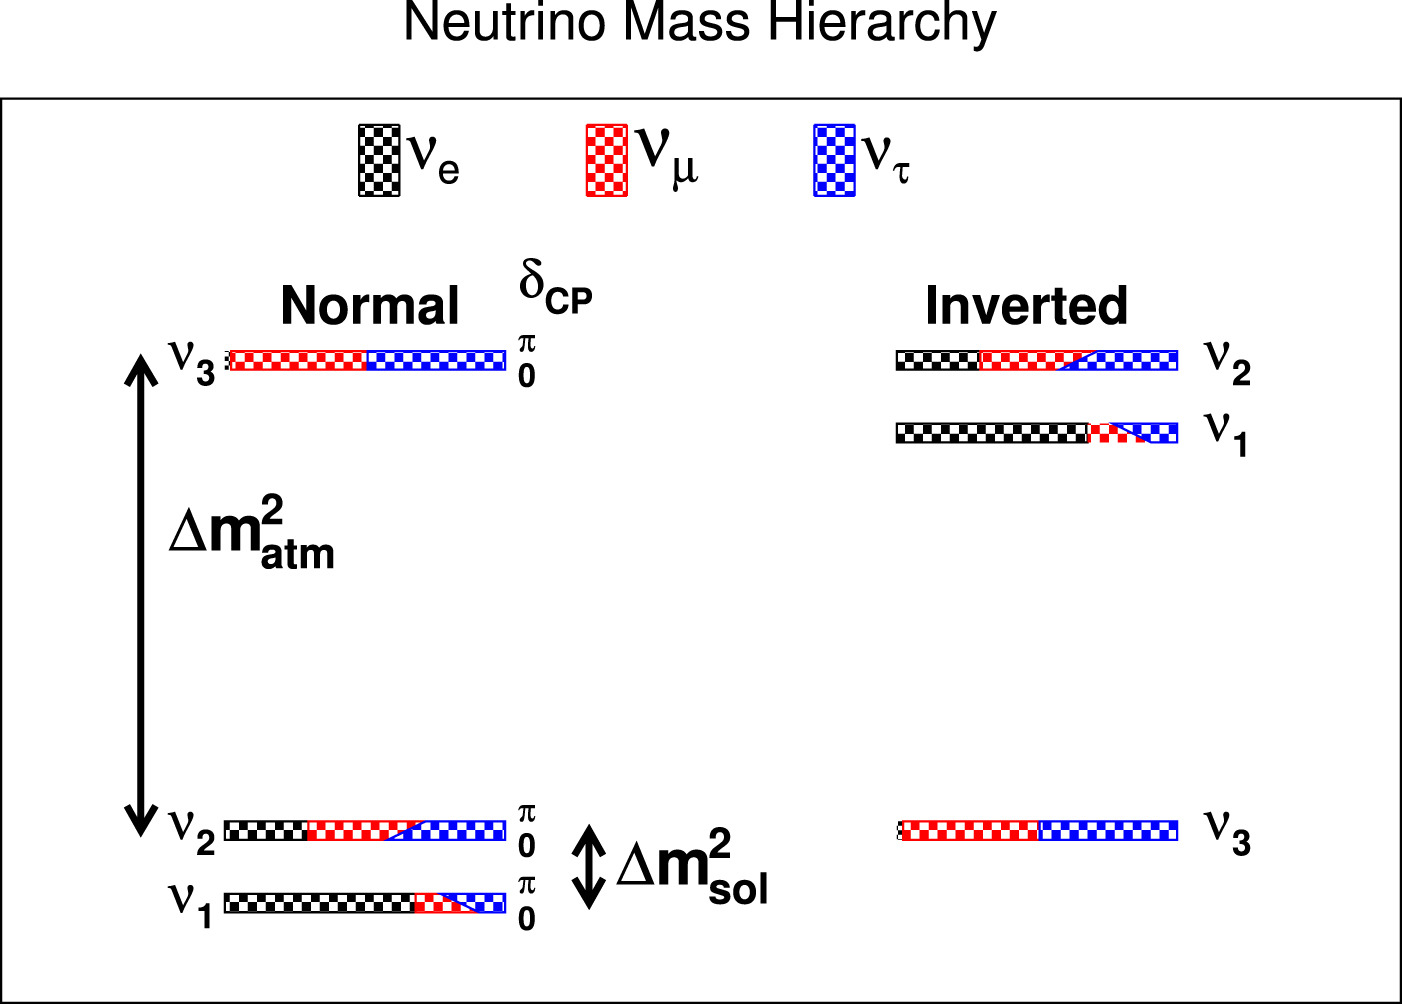
\includegraphics[width=\textwidth]{images/mass_hierarchy.jpg}
\caption{Representation of the mass hierarchy scales. This is a represntation of the two possible orderings of neutrino massses, due to the uncertain sign of $m_{13}$. It is also interesting to observe that the absolute mass scale is not measured since oscillation measurements only give difference mass squares. Image was taken from~\citep{QIAN20151}.}
\end{figure}~\label{fig:mass_hierarchy}

Neutrino oscillations in matter are slightly different than those in vacuum~\citep{PhysRevD.17.2369}.
The Mikheyev-Smirnov-Wolfenstein (MSW) effect~\citep{Smirnov2004TheME} also contributes to differening neutrino oscillations as they move through matter of varying density, which additionally complicated the calculation.
The MSW effect also affects neutrinos differently than anti-neutrinos, which is useful for measuring $\delta_{cp}$.
This resonance affect for beam-line experiments affects $\nu_{e}$ in the case of normal mass ordering (NO), whereas in the case of inverted mass order (IO), the $\hat{\nu_{e}}$ experiences resonance and is thus more likely.

\begin{table}
\begin{center}
\begin{tabular}{||c c c c||}
 \hline
 Paramater & Best Fit & Unit & Best Soruce\\ [0.5ex]
 \hline\hline
  $\theta_{13}$ & $8.57^{+0.12}_{-0.12}$ & na & Reactor \\ % DAYA/doubleChooz/RENO 2012 Daya Bay found not equal to zero
 \hline
  $\theta_{12}$ & $33.44^{+0.77}_{-0.74}$ & Atmospheric \\ % KamLAND + SNO, liquid scintillator
 \hline
  $\theta_{23}$ & $49.2^{+0.9}_{-1.2}$ & na & Solar \\ % Solar, T2k(water cherenkov) / NOvA(liquid scintillator / numi off axis)
 \hline
  $\delta_{cp}$ & $197^{+27}_{-24}$ & na & Atmospheric+Accelerator \\ % t2k / NOva, https://pdg.lbl.gov/2022/listings/rpp2022-list-neutrino-mixing.pdf
 \hline
  $\Delta m_{21}^{2}$ & $7.42^{0.21}_{-0.20}$ & $10^{-5}eV^{2}$ & Solar \\ % kamland / SNO / SKAM
 \hline
  $\Delta m_{3l}^{2}$ & $2.517^{+0.026}_{-0.028}$ & $10^{-3}eV^{2}$ & Atmospheric  \\
 \hline
\end{tabular}
\caption{Known Oscillation Parameters of Interest. Values are taken from the global fit~\citep{2020JHEP...09..178E}. The values shown assume normal mass ordering for neutrinos and include atmospheric Super-Kamikonde Data.}
\end{center}
\end{table}
~\label{table:pmns_params}


\section{Neutrino Tracking Detectors in the Current Century}

Finally, in this last section we discuss the development of various upcoming detector technologies.
There are many motivating pressures for new detectors to adopt pixelated designs. 
Below we discuss two contributing factors: the development of electronics and computing algorithms.

First, previously pixelated detectors have historically been more difficult because of the issues of cost and size regarding the number of readout channels.
This is being addressed, in part, by the advent of newer, cheaper, and larger Field-Programmable-Gate Arrays (FPGAs).
One method for reducing the electronic overhead required in pixelated detectors is to use digital multiplexing.
Cheap, high channel FPGAs directly solve this problem. 
Other electronics development, such as the Silicon-Photomultiplier, offer much cheaper alternatives for large pixel counters compared to their historical counter-parts.

\begin{table}
\begin{center}
\begin{tabular}{||c c c||}
 \hline
 Paramater & Best Experiments & Type of Detector \\ [0.5ex]
 \hline\hline
  $\theta_{13}$ & & \\
 \hline
  $\theta_{12}$ & & \\
 \hline
  $\theta_{23}$ & & \\
 \hline
  $\delta_{cp}$ & & \\
 \hline
  $\Delta m_{21}^{2}$ & & \\
 \hline
  $\Delta m_{3l}^{2}$ & & \\
 \hline
\end{tabular}
\caption{Comparison of which type of detectors are useful for measuring which values of neutrino oscillation.}
\end{center}
\end{table}
~\label{table:pmns_detectors}

\section{Future Detectors}

%% antihydrogen
\citep{Sadowski_2017}
Another driving factor is the the development of Machine Learning (ML) algorithms, particularly Convectional Neural Network (CNN \citep{Sadowski2017DeepLI}).
Recent industry has driven the need for CNNs to be able to correctly identify and label 2-D images of various kinds, and thus championed much of progress in this field and spawned many kinds of CNN algorithms.

%% cite sadowski here
Recently, it has been shown how these kinds of algorithms extend into High Energy Physics (HEP) for particle identification.
A major issue at the Intensity Frontier of physics is the sheer amount of data to store and process.
These ML algorithms provied a developed tool to automate the analysis of huge amounts of data ($>> 1 TB$) and have been shown to be quite accurate ($>99\%$) at particle identification in LArTPCs.


%% LArPix / Argon Cube
Additional work has been performed in recent years which show that LArTPCs can also utilized a pixel-based readout~\citep{larpix:Dwyer_2018}, \citep{Asaadi_2018}.

The end of the Standard Model era is inevitable.
SM simply fails to account for physics with all major frontiers for physicists to accept its completeness; we know there is much and more to learn about nature.

The 20th century saw unprecedented progress in its sophistication of its detectors from ray tubes, to spark chambers, to proportional counters, and to huge (>20 km) particle accelerators.
This century shows no signs holding any less promise than its predecessor.
Continued development in electronics, computing, and analysis methods will lead to more and newer frontiers of physics.

The work presented in this introduction aims to not only encapsulate the massive progress particle physics has made since the electron's discovery, but also to server as a reminder of how extraordinarily surprising nature is.
At every turn and at every point where physicists think they've arrived at the end (or at an impossible roadblock) there always remains more to discover.
If we have learned anything, we have learned to knock and the door shall be opened.


%% Highlight what DUNE is and its purpose
\subsection{The Deep Underground Neutrino Experiment}~\label{sec:dune}

The Deep Underground Neutrino Experiment (DUNE) is a long-baseline neutrino beam experiment~\citep{DUNE_TDR_V1_Abi_2020, DUNE_FD_TDRv2_2020, DUNE_TDRv3_Abi_2020, DUNE-FD_TDRv4:Abi_2020}.
DUNE, when constructed, will be composed two detectors, a near detector (ND) and a far detector (FD) which are separated by a distance of 1300 km.

The ND is located at Fermilab and its purpose is to characterize the source neutrino beam created there.
The ND serves many purposes.
To name a few..TODO

The FD will be placed underground at Sanford Underground Research Facility (SURF) and be approximately 1300 km away from the ND.
This detector represents an enormous engineering challenge to place such large, cold, and complicated detector.
The FD will be composed of up to four separate 10 kiloton modules.

DUNE plans to offer an incredibly rich searches across the sectors listed above~\ref{item:dune_props}.
We briefly discuss the relevance of some the searches below, but more detailed reading can be pursued at~\citep{DUNE_FD_TDRv2_2020}.

Two of these four modules at least will use a known wire-based readout technology and a vertical drift-readout.
The two remaining modules are considered modules of opportunity and their readout technology is yet unknown.
A purpose of this dissertation is show the viability of a novel readout technology.

\begin{figure}[]
\centering
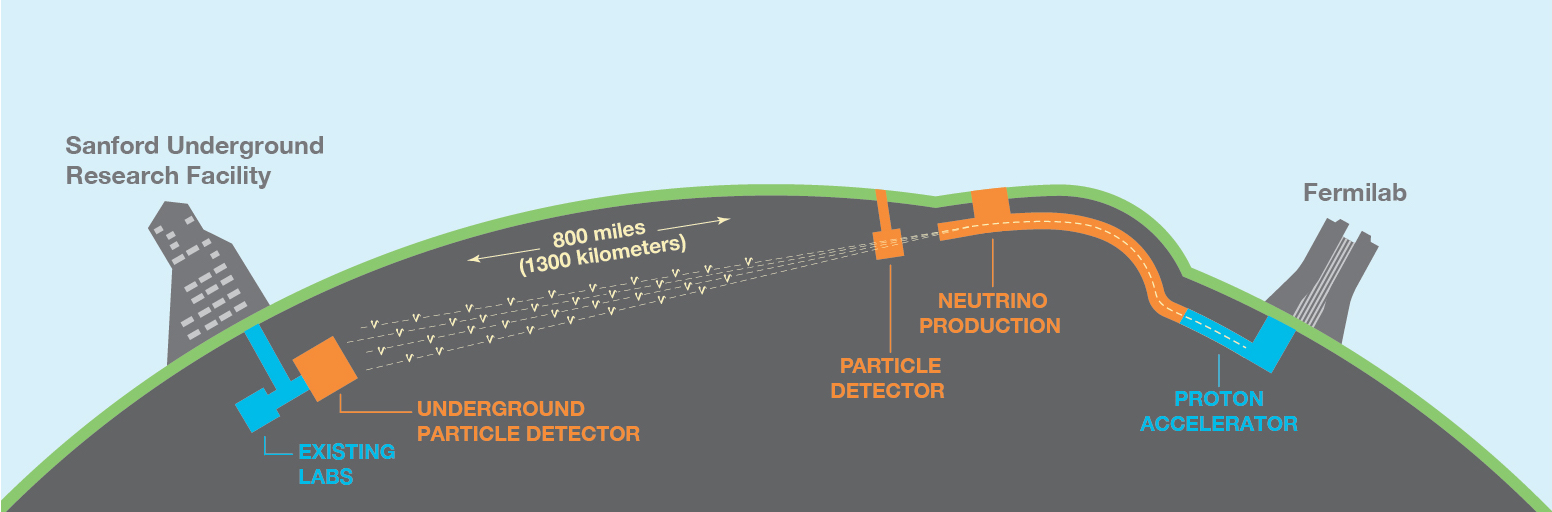
\includegraphics[width=\textwidth]{images/LBNE_Graphic_061615_2016.jpg}
\caption{Representation of the Near and Far Detectors for the DUNE experiment. The Near Detector is located within the image labeled as the Particle Detector. One of the key purposes for the Near Detector is to tag outgoing particles from the proton beam. Image was taken from~\citep{dune_cdr_2016_arxiv}.}
\end{figure}

DUNE has three main science goals, all of which are geared towards pushing beyond the standard model:
\begin{itemize}
    \item Hadron Decay~\ref{sec:hadron_decay}
    \item Core-collapse Supernovae~\ref{sec:intro_supernova}
    \item Neutrino Oscillation~\ref{sec:neutrino_osc}
\end{itemize}
~\label{item:dune_props}

We will discuss the relevance of each of these items, and in chapter~\ref{chap:qpix} where we will further discuss how the work presented here relates to each of these topics.

Conventional horizontal drift detection for foreseeable DUNE modules are already considered possible for lengths up to 6.5m \citep{DUNE_Vertical:Paulucci_2022}.